\documentclass[12pt]{article}

% =========================
% Geometry & core packages
% =========================
\usepackage[a4paper,margin=0.8in]{geometry}
\usepackage{amsmath,amssymb,amsthm,mathtools}
\usepackage{bm}
\usepackage{array,booktabs}
\usepackage{enumitem}
\usepackage{microtype}
\usepackage{xcolor}
\usepackage{hyperref}
\usepackage{fancyhdr}
\usepackage{draftwatermark}
\usepackage{tikz}
% =========================
% Watermark (consistent style)
% =========================
\SetWatermarkText{Unofficial — QRS@NTU — qrsntu.org}
\SetWatermarkScale{1}
\SetWatermarkLightness{0.99}

% =========================
% Course metadata
% =========================
\newcommand{\CourseCode}{MH1101}
\newcommand{\CourseName}{Calculus II}
\newcommand{\DocType}{Midterm Test (Solutions)}
\newcommand{\ExamMeta}{AY 2017/2018, Semester 2}
\newcommand{\ExamMetaShort}{Midterm AY17-18 Sem 2}

\title{
\Huge \CourseCode\ \CourseName \\[0.3em]
\Large \DocType \\[0.3em]
\large \ExamMeta
}
\author{
  \textit{\href{https://qrsntu.org}{Quantitative Research Society @NTU}}
}
\date{\today}

% =========================
% Header/footer styles
% =========================
\fancypagestyle{main}{
  \fancyhf{}
  \fancyhead[L]{\CourseCode\ \CourseName\ --\ \ExamMetaShort}
  \fancyhead[R]{\href{https://qrsntu.org}{QRS@NTU}}
  \fancyfoot[C]{\thepage}
  \renewcommand{\headrulewidth}{0.4pt}
  \renewcommand{\footrulewidth}{0pt}
}

\fancypagestyle{plainfirst}{
  \fancyhf{}
  \renewcommand{\headrulewidth}{0pt}
  \renewcommand{\footrulewidth}{0pt}
  \fancyfoot[C]{\scriptsize\textcolor{gray}{\textit{For academic reference only. This document is provided for educational purposes and does not constitute an official question paper, answer key, or any formally authorised academic material. Its content is not guaranteed to be complete or accurate.}}}
}

% =========================
% Convenience macros
% =========================
\newcommand{\dd}{\,\mathrm{d}}
\newcommand{\ee}{\mathrm{e}}
\newcommand{\ii}{\mathrm{i}}
\newcommand{\R}{\mathbb{R}}
\newcommand{\N}{\mathbb{N}}

% Overview block
\newenvironment{overview}{
  \par\bigskip
  \begin{center}
    \rule{0.92\linewidth}{0.6pt}\\[-0.2em]
    \textbf{Overview}\\[-0.2em]
    \rule{0.92\linewidth}{0.6pt}
  \end{center}
  \vspace{-0.3em}
  \begin{itemize}[leftmargin=1.6em, itemsep=0.2em, topsep=0.2em]
}{
  \end{itemize}
  \par\bigskip
}

\usepackage{titlesec}

\titleformat{\subsubsection}[block]
{\normalfont\large\bfseries}
{}
{0pt}
{}

\titleformat{\paragraph}[block]
{\normalfont\normalsize\bfseries}
{}
{0pt}
{}

\titlespacing*{\paragraph}
{0pt}      % left margin
{1.2ex}    % space before
{0.6ex}    % space after

\setlist[enumerate]{itemsep=0.3em, topsep=0.3em}
\setlist[itemize]{itemsep=0.2em, topsep=0.2em}

\setcounter{secnumdepth}{-1}
\setcounter{tocdepth}{4}



\begin{document}

\maketitle
\thispagestyle{plainfirst}
\pagestyle{main}

\begin{overview}
  \item Fundamental Theorem of Calculus and differentiation of integrals with variable limits.
  \item Riemann sums and their interpretation as definite integrals.
  \item Applications of integration: volumes of solids of revolution via cylindrical shells and washers.
  \item Techniques of integration: trigonometric identities, substitutions, and integration by parts.
\end{overview}

\newpage
\tableofcontents
\newpage

\section[Question 1 (16 marks)]{Question 1 \hfill (16 marks)}

\subsection{(a) Derivative of an integral with variable limits \hfill (8 marks)}

\[
\frac{\dd}{\dd x}\int_x^{x^2}\sin(t^2)\,\dd t
\]

\subsubsection{Solution}

\paragraph{Method 1: Direct application of the Leibniz rule}
Let
\[
F(x)=\int_x^{x^2}\sin(t^2)\,\dd t.
\]
By the Leibniz rule,
\[
\frac{\dd}{\dd x}\int_{u(x)}^{v(x)} f(t)\,\dd t
=f(v(x))\,v'(x)-f(u(x))\,u'(x).
\]
Here,
\[
f(t)=\sin(t^2),\qquad u(x)=x,\qquad v(x)=x^2.
\]
Hence
\[
F'(x)=\sin\bigl((x^2)^2\bigr)\cdot 2x-\sin(x^2)\cdot 1
=2x\sin(x^4)-\sin(x^2).
\]
Therefore
\[
\boxed{
\frac{\dd}{\dd x}\int_x^{x^2}\sin(t^2)\,\dd t
=2x\sin(x^4)-\sin(x^2).
}
\]

\paragraph{Method 2: Rewrite using a fixed lower limit}
Define
\[
G(y)=\int_0^y \sin(t^2)\,\dd t.
\]
Then
\[
\int_x^{x^2}\sin(t^2)\,\dd t=G(x^2)-G(x).
\]
By the Fundamental Theorem of Calculus,
\(
G'(y)=\sin(y^2).
\)
Hence, by the chain rule,
\[
\frac{\dd}{\dd x}\bigl(G(x^2)-G(x)\bigr)
=G'(x^2)\cdot 2x-G'(x)
=2x\sin(x^4)-\sin(x^2).
\]
So again,
\[
\boxed{
\frac{\dd}{\dd x}\int_x^{x^2}\sin(t^2)\,\dd t
=2x\sin(x^4)-\sin(x^2).
}
\]

\subsubsection{Marking scheme}
\begin{itemize}
\item 2 marks: Correct identification of the relevant rule (Leibniz rule or equivalent FTC decomposition).
\item 2 marks: Correct substitution of the upper and lower limits into \(\sin(t^2)\).
\item 2 marks: Correct differentiation of the limits, giving factors \(2x\) and \(1\).
\item 2 marks: Correct simplification to \(2x\sin(x^4)-\sin(x^2)\).
\end{itemize}

\newpage
\subsection{(b) Writing a limit as a definite integral \hfill (8 marks)}

\[
\lim_{n\to\infty}\sum_{i=1}^{n}\frac{1}{n}\left(1+\frac{4i}{n}\right)^3
\]

\subsubsection{Solution}

\paragraph{Method 1: Direct Riemann-sum recognition}
Write
\[
\sum_{i=1}^{n}\frac{1}{n}\left(1+\frac{4i}{n}\right)^3
=\sum_{i=1}^{n} f\!\left(\frac{i}{n}\right)\Delta x,
\qquad
f(x)=(1+4x)^3,\quad \Delta x=\frac{1}{n}.
\]
This is the right-endpoint Riemann sum for \(f(x)=(1+4x)^3\) on the interval \([0,1]\).
Therefore
\[
\lim_{n\to\infty}\sum_{i=1}^{n}\frac{1}{n}\left(1+\frac{4i}{n}\right)^3
=\int_0^1 (1+4x)^3\,\dd x.
\]
Thus
\[
\boxed{
\lim_{n\to\infty}\sum_{i=1}^{n}\frac{1}{n}\left(1+\frac{4i}{n}\right)^3
=\int_0^1 (1+4x)^3\,\dd x.
}
\]

\paragraph{Method 2: Rewrite the sample points}
Set
\[
u_i=1+\frac{4i}{n}.
\]
Then consecutive terms satisfy
\[
\Delta u=u_i-u_{i-1}=\frac{4}{n},
\qquad
\frac{1}{n}=\frac{1}{4}\Delta u.
\]
Hence
\[
\sum_{i=1}^{n}\frac{1}{n}\left(1+\frac{4i}{n}\right)^3
=\frac{1}{4}\sum_{i=1}^{n} u_i^3\,\Delta u.
\]
As \(n\to\infty\), this is the Riemann sum for
\[
\frac14\int_1^5 u^3\,\dd u.
\]
Therefore
\[
\boxed{
\lim_{n\to\infty}\sum_{i=1}^{n}\frac{1}{n}\left(1+\frac{4i}{n}\right)^3
=\frac14\int_1^5 u^3\,\dd u.
}
\]
This is equivalent to \(\int_0^1 (1+4x)^3\,\dd x\).

\subsubsection{Marking scheme}
\begin{itemize}
\item 2 marks: Correct recognition of the expression as a Riemann sum.
\item 2 marks: Correct interval and sample points, e.g. \([0,1]\) with \(x_i=i/n\).
\item 2 marks: Correct identification of the integrand \((1+4x)^3\) or an equivalent integrand under a valid change of variable.
\item 2 marks: Correct final definite integral, without evaluation.
\end{itemize}

\newpage

\section[Question 2 (16 marks)]{Question 2 \hfill (16 marks)}

\subsection{(a) Volume of a solid of revolution \hfill (8 marks)}

Let \(R\) be the region bounded by the lines \(y=x\), \(y=4-x\) and \(y=0\) in the first quadrant. Compute the volume of the solid formed by revolving \(R\) about the line \(x=-1\).

\subsubsection{Solution}

\paragraph{Method 1: Cylindrical shells}

\begin{center}
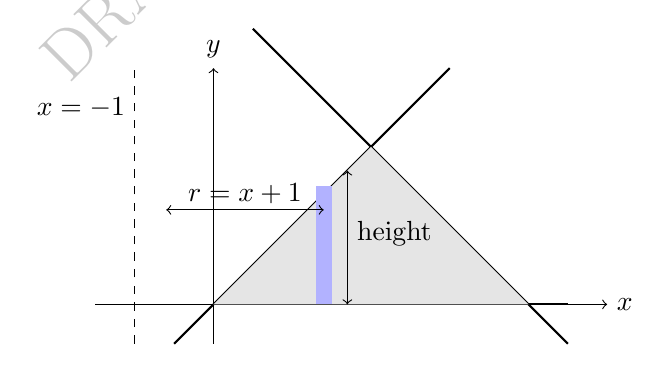
\begin{tikzpicture}[scale=1.0]

% Axes
\draw[->] (-1.5,0) -- (5,0) node[right] {$x$};
\draw[->] (0,-0.5) -- (0,3) node[above] {$y$};

% Axis of rotation
\draw[dashed] (-1,-0.5) -- (-1,3);
\node[left] at (-1,2.5) {$x=-1$};

% Lines
\draw[thick,domain=-0.5:3] plot (\x,\x);
\draw[thick,domain=0.5:4.5] plot (\x,{4-\x});
\draw[thick] (0,0) -- (4.5,0);

% Shaded region
\fill[gray!20] (0,0) -- (2,2) -- (4,0) -- cycle;

% Shell strip
\fill[blue!30] (1.3,0) rectangle (1.5,1.5);

% Radius arrow
\draw[<->] (-0.6,1.2) -- (1.4,1.2);
\node at (0.4,1.4) { $r=x+1$};

% Height arrow
\draw[<->] (1.7,0) -- (1.7,1.7);
\node[right] at (1.7,0.9) {height};

\end{tikzpicture}
\end{center}
Since the axis of rotation is the vertical line \(x=-1\), the shell method with respect to \(x\) is natural.

For \(0\le x\le 2\), the top curve is \(y=x\), so the shell height is \(x\).
For \(2\le x\le 4\), the top curve is \(y=4-x\), so the shell height is \(4-x\).
In both cases, the shell radius is the horizontal distance from \(x\) to \(x=-1\), namely \(x+1\).

Therefore
\[
V=2\pi\left(\int_0^2 (x+1)x\,\dd x+\int_2^4 (x+1)(4-x)\,\dd x\right).
\]
Now
\[
\int_0^2 (x+1)x\,\dd x
=\int_0^2 (x^2+x)\,\dd x
=\left[\frac{x^3}{3}+\frac{x^2}{2}\right]_0^2
=\frac{8}{3}+2
=\frac{14}{3},
\]
and
\[
\int_2^4 (x+1)(4-x)\,\dd x
=\int_2^4 (-x^2+3x+4)\,\dd x
=\left[-\frac{x^3}{3}+\frac{3x^2}{2}+4x\right]_2^4
=\frac{22}{3}.
\]
Hence
\[
V=2\pi\left(\frac{14}{3}+\frac{22}{3}\right)=2\pi(12)=24\pi.
\]
So the required volume is
\[
\boxed{V=24\pi.}
\]
\newpage
\paragraph{Method 2: Washers}
Express the triangular region in terms of \(y\).



For \(0\le y\le 2\), the left boundary is \(x=y\) and the right boundary is \(x=4-y\).
After revolving about \(x=-1\), a horizontal strip gives a washer with
\[
R(y)=(4-y)-(-1)=5-y,
\qquad
r(y)=y-(-1)=y+1.
\]
Therefore
\[
V=\pi\int_0^2 \bigl(R(y)^2-r(y)^2\bigr)\,\dd y
=\pi\int_0^2 \bigl((5-y)^2-(y+1)^2\bigr)\,\dd y.
\]
Simplifying,
\[
(5-y)^2-(y+1)^2
=(25-10y+y^2)-(y^2+2y+1)
=24-12y.
\]
Hence
\[
V=\pi\int_0^2 (24-12y)\,\dd y
=\pi\left[24y-6y^2\right]_0^2
=\pi(48-24)
=24\pi.
\]
Thus
\[
\boxed{V=24\pi.}
\]

\subsubsection{Marking scheme}
\begin{itemize}
\item 2 marks: Correct geometric setup of the region and correct choice of a valid method (shells or washers).
\item 2 marks: Correct radius and height / outer radius and inner radius.
\item 2 marks: Correct integral setup, including correct limits and any splitting if needed.
\item 2 marks: Correct evaluation leading to \(V=24\pi\).
\end{itemize}


\subsection{(b) Describing a solid from a volume integral \hfill (8 marks)}

Describe a solid of revolution whose volume is given by the definite integral
\[
\int_{-2}^{4} 2\pi(y+3)\bigl(9-(y-1)^2\bigr)\,\dd y.
\]

\subsubsection{Solution}

\paragraph{Method 1: Direct shell-method interpretation}
The formula
\[
\int_{-2}^{4} 2\pi(y+3)\bigl(9-(y-1)^2\bigr)\,\dd y
\]
has the shell-method form
\[
\int_a^b 2\pi\,(\text{radius})(\text{height})\,\dd y.
\]
Thus the shells are horizontal, so the axis of rotation is a horizontal line.

The radius is \(y+3\), which is the distance from \(y\) to the line \(y=-3\).
The height is \(9-(y-1)^2\), which is the horizontal length from \(x=0\) to the curve
\[
x=9-(y-1)^2.
\]
Also, the bounds \(-2\le y\le 4\) are exactly the values for which \(9-(y-1)^2\ge 0\).

\[
\boxed{
\begin{aligned}
&\text{The solid obtained by revolving the region }\\
&\{(x,y)\mid -2\le y\le 4,\ 0\le x\le 9-(y-1)^2\}\\
&\text{about the line }y=-3.
\end{aligned}
}
\]

\paragraph{Method 2: Geometric reconstruction from the generating curve}
Observe that
\[
x=9-(y-1)^2
\]
is a left-opening parabola with vertex \((9,1)\). Its intersections with the line \(x=0\) satisfy
\[
0=9-(y-1)^2
\quad\Longleftrightarrow\quad
(y-1)^2=9
\quad\Longleftrightarrow\quad
y=-2 \text{ or } y=4.
\]
Hence the planar region is the region between the parabola
\[
x=9-(y-1)^2
\]
and the \(y\)-axis \(x=0\), for \(-2\le y\le 4\).

Since the factor \(y+3\) gives the distance from \(y\) to \(y=-3\), the axis of revolution is the horizontal line
\[
y=-3.
\]
Therefore one valid description is:
\[
\boxed{
\begin{aligned}
&\text{The solid obtained by revolving the region enclosed by }\\
&x=0 \text{ and } x=9-(y-1)^2,\quad -2\le y\le 4,\\
&\text{about the line }y=-3.
\end{aligned}
}
\]

\paragraph{Alternative equivalent description}
Rewrite the parabola as
\[
(y-1)^2=9-x.
\]
Then for \(0\le x\le 9\), the upper and lower branches are
\[
y=1+\sqrt{9-x},
\qquad
y=1-\sqrt{9-x}.
\]
Thus the same region may also be described as
\[
\{(x,y)\mid 0\le x\le 9,\ 1-\sqrt{9-x}\le y\le 1+\sqrt{9-x}\},
\]
and the solid is obtained by revolving this region about the line \(y=-3\).

\subsubsection{Marking scheme}
\begin{itemize}
\item 2 marks: Correct recognition that the integral is a shell-method volume formula in \(y\).
\item 2 marks: Correct axis of rotation \(y=-3\).
\item 2 marks: Correct identification of the generating region, e.g. \(0\le x\le 9-(y-1)^2\) for \(-2\le y\le 4\).
\item 2 marks: Clear and mathematically complete verbal or symbolic description of the solid.
\end{itemize}

\newpage
\section[Question 3 (18 marks)]{Question 3 \hfill (18 marks)}

Evaluate the following integrals.

\subsection{(a) Trigonometric integral \hfill (6 marks)}

\[
\int \sec^5(2x)\tan^3(2x)\,\dd x
\]

\bigskip
\subsubsection{Solution}

\paragraph{Method 1: Standard direct method}
Use
\[
\tan^2(2x)=\sec^2(2x)-1.
\]
Then
\begin{align*}
\int \sec^5(2x)\tan^3(2x)\,\dd x
&=\int \sec^5(2x)\tan(2x)\tan^2(2x)\,\dd x \\
&=\int \sec^5(2x)\tan(2x)\bigl(\sec^2(2x)-1\bigr)\,\dd x \\
&=\int \bigl(\sec^6(2x)-\sec^4(2x)\bigr)\sec(2x)\tan(2x)\,\dd x.
\end{align*}
Let
\[
u=\sec(2x).
\]
Then
\[
\dd u=2\sec(2x)\tan(2x)\,\dd x,
\qquad
\sec(2x)\tan(2x)\,\dd x=\frac12\,\dd u.
\]
Therefore
\begin{align*}
\int \sec^5(2x)\tan^3(2x)\,\dd x
&=\frac12\int (u^6-u^4)\,\dd u \\
&=\frac12\left(\frac{u^7}{7}-\frac{u^5}{5}\right)+C \\
&=\frac{1}{14}\sec^7(2x)-\frac{1}{10}\sec^5(2x)+C.
\end{align*}
Hence
\[
\boxed{
\int \sec^5(2x)\tan^3(2x)\,\dd x
=\frac{1}{14}\sec^7(2x)-\frac{1}{10}\sec^5(2x)+C.
}
\]

\newpage
\paragraph{Method 2: Faster parity-based method}

Since the power of \(\tan\) is odd, write
\[
\int \sec^5(2x)\tan^3(2x)\,\dd x
=\int \sec^4(2x)\tan^2(2x)\,\sec(2x)\tan(2x)\,\dd x.
\]
Using
\[
\tan^2(2x)=\sec^2(2x)-1,
\]
this becomes
\[
\int \sec^4(2x)\bigl(\sec^2(2x)-1\bigr)\sec(2x)\tan(2x)\,\dd x.
\]
Let
\[
u=\sec(2x).
\]
Then
\[
\dd u=2\sec(2x)\tan(2x)\,\dd x.
\]
Hence
\begin{align*}
\int \sec^5(2x)\tan^3(2x)\,\dd x
&=\frac12\int u^4(u^2-1)\,\dd u \\
&=\frac12\int (u^6-u^4)\,\dd u \\
&=\frac{1}{14}u^7-\frac{1}{10}u^5+C.
\end{align*}
Therefore
\[
\boxed{
\int \sec^5(2x)\tan^3(2x)\,\dd x
=\frac{1}{14}\sec^7(2x)-\frac{1}{10}\sec^5(2x)+C.
}
\]

\subsubsection{Marking scheme}
\begin{itemize}
\item 2 marks: Correct trigonometric rewriting, e.g. using \(\tan^2(2x)=\sec^2(2x)-1\) or an equivalent identity.
\item 2 marks: Correct substitution and transformed integrand.
\item 2 marks: Correct antiderivative
\[
\frac{1}{14}\sec^7(2x)-\frac{1}{10}\sec^5(2x)+C.
\]
\end{itemize}

\newpage
\subsection{(b) Logarithmic integral \hfill (6 marks)}

\[
\int \frac{\ln(2x)}{x^2}\,\dd x
\]
\bigskip
\subsubsection{Solution}

\paragraph{Method 1: Integration by parts}

Use integration by parts. Let
\[
u=\ln(2x),
\qquad
\dd v=x^{-2}\,\dd x.
\]
Then
\[
\dd u=\frac{1}{x}\,\dd x,
\qquad
v=-x^{-1}=-\frac{1}{x}.
\]
Thus
\begin{align*}
\int \frac{\ln(2x)}{x^2}\,\dd x
&=uv-\int v\,\dd u \\
&=-\frac{\ln(2x)}{x}-\int\left(-\frac{1}{x}\right)\left(\frac{1}{x}\right)\dd x \\
&=-\frac{\ln(2x)}{x}+\int x^{-2}\,\dd x \\
&=-\frac{\ln(2x)}{x}-\frac{1}{x}+C.
\end{align*}
Therefore
\[
\boxed{
\int \frac{\ln(2x)}{x^2}\,\dd x
=-\frac{\ln(2x)+1}{x}+C.
}
\]
\bigskip
\paragraph{Method 2: Derivative-recognition method}

Observe that
\[
\frac{\dd}{\dd x}\left(\frac{\ln(2x)}{x}\right)
=\frac{(1/x)\cdot x-\ln(2x)}{x^2}
=\frac{1-\ln(2x)}{x^2}.
\]
Hence
\[
\frac{\ln(2x)}{x^2}
=\frac{1}{x^2}-\frac{\dd}{\dd x}\left(\frac{\ln(2x)}{x}\right).
\]
Integrating both sides,
\begin{align*}
\int \frac{\ln(2x)}{x^2}\,\dd x
&=\int x^{-2}\,\dd x-\int \frac{\dd}{\dd x}\left(\frac{\ln(2x)}{x}\right)\dd x \\
&=-\frac{1}{x}-\frac{\ln(2x)}{x}+C.
\end{align*}
Therefore
\[
\boxed{
\int \frac{\ln(2x)}{x^2}\,\dd x
=-\frac{\ln(2x)+1}{x}+C.
}
\]

\bigskip
\subsubsection{Marking scheme}
\begin{itemize}
\item 2 marks: Correct setup of integration by parts or an equivalent derivative-based decomposition.
\item 2 marks: Correct intermediate algebra and evaluation of the remaining integral.
\item 2 marks: Correct final answer
\[
-\frac{\ln(2x)+1}{x}+C.
\]
\end{itemize}
\bigskip
\subsection{(c) Definite integral with symmetry \hfill (6 marks)}

\[
\int_0^1 \frac{\sin x}{\sin(1-x)+\sin x}\,\dd x
\qquad
\text{(Hint: }u=1-x\text{)}
\]
\bigskip
\subsubsection{Solution}

\paragraph{Method 1: Direct use of the given hint}

Let
\[
I=\int_0^1 \frac{\sin x}{\sin(1-x)+\sin x}\,\dd x.
\]
Use the substitution
\[
u=1-x.
\]
Then
\[
\dd u=-\dd x,
\qquad
x=0\Rightarrow u=1,
\qquad
x=1\Rightarrow u=0.
\]
So
\begin{align*}
I
&=\int_1^0 \frac{\sin(1-u)}{\sin u+\sin(1-u)}(-\dd u) \\
&=\int_0^1 \frac{\sin(1-u)}{\sin u+\sin(1-u)}\,\dd u.
\end{align*}
Renaming \(u\) as \(x\), we get
\[
I=\int_0^1 \frac{\sin(1-x)}{\sin x+\sin(1-x)}\,\dd x.
\]
Adding this to the original expression for \(I\),
\begin{align*}
2I
&=\int_0^1 \frac{\sin x+\sin(1-x)}{\sin(1-x)+\sin x}\,\dd x \\
&=\int_0^1 1\,\dd x=1.
\end{align*}
Hence
\[
I=\frac12.
\]
Therefore
\[
\boxed{
\int_0^1 \frac{\sin x}{\sin(1-x)+\sin x}\,\dd x=\frac12.
}
\]

\paragraph{Method 2: Symmetry recognition}

Recognize the symmetry pattern
\[
\int_a^b \frac{f(x)}{f(x)+f(a+b-x)}\,\dd x=\frac{b-a}{2},
\]
provided the denominator is nonzero on \([a,b]\).

Indeed, under the substitution \(u=a+b-x\), the same integral becomes
\[
\int_a^b \frac{f(a+b-x)}{f(x)+f(a+b-x)}\,\dd x,
\]
and adding the two expressions gives
\[
2\int_a^b \frac{f(x)}{f(x)+f(a+b-x)}\,\dd x
=\int_a^b 1\,\dd x=b-a.
\]

Here,
\[
a=0,\qquad b=1,\qquad f(x)=\sin x,
\]
so
\[
\int_0^1 \frac{\sin x}{\sin x+\sin(1-x)}\,\dd x
=\frac{1-0}{2}
=\frac12.
\]
Therefore
\[
\boxed{
\int_0^1 \frac{\sin x}{\sin(1-x)+\sin x}\,\dd x=\frac12.
}
\]
\bigskip
\subsubsection{Marking scheme}
\begin{itemize}
\item 2 marks: Correct use of the substitution \(u=1-x\) or an equivalent symmetry argument.
\item 2 marks: Correct formation of the equation \(2I=1\) or an equivalent simplification.
\item 2 marks: Correct final value
\[
I=\frac12.
\]
\end{itemize}
\end{document}